\subsection{Averaging Filter}
See Figure~\ref{fig:2-1-1} for the results from applying the averaging filter to the test image with salt \& pepper noise applied, and Figure~\ref{fig:2-1-2} for the ones for the test image with Gaussian noise applied to it.
The original noisy images are displayed for comparison.

\begin{figure}[h]
    \centering

    \begin{subfigure}[b]{0.3\textwidth}
        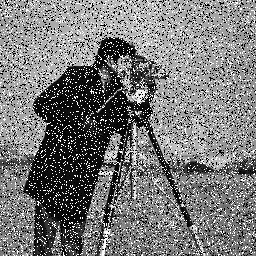
\includegraphics[width=0.9\textwidth]{../code/2_out/2-1_sp.png}
        \caption{No filter.}
        \label{fig:2-1-1:1}
    \end{subfigure}
    \begin{subfigure}[b]{0.3\textwidth}
        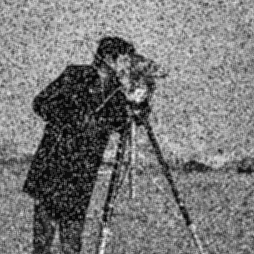
\includegraphics[width=0.9\textwidth]{../code/2_out/2-1_sp_3x3.png}
        \caption{3x3}
        \label{fig:2-1-1:2}
    \end{subfigure}

    \begin{subfigure}[b]{0.3\textwidth}
        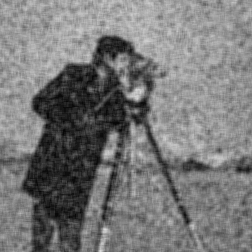
\includegraphics[width=0.9\textwidth]{../code/2_out/2-1_sp_5x5.png}
        \caption{5x5}
        \label{fig:2-1-1:3}
    \end{subfigure}
    \begin{subfigure}[b]{0.3\textwidth}
        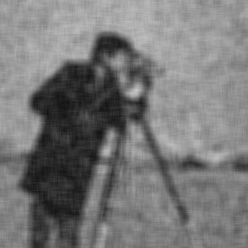
\includegraphics[width=0.9\textwidth]{../code/2_out/2-1_sp_9x9.png}
        \caption{9x9}
        \label{fig:2-1-1:4}
    \end{subfigure}

    \caption{Averaging filter of varying sizes applied to image with salt \& pepper noise.}
    \label{fig:2-1-1}
\end{figure}


\begin{figure}[h]
    \centering

    \begin{subfigure}[b]{0.3\textwidth}
        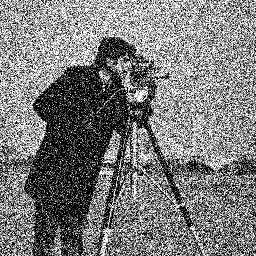
\includegraphics[width=0.9\textwidth]{../code/2_out/2-1_gaus.png}
        \caption{No filter.}
        \label{fig:2-1-2:1}
    \end{subfigure}
    \begin{subfigure}[b]{0.3\textwidth}
        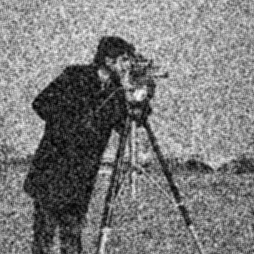
\includegraphics[width=0.9\textwidth]{../code/2_out/2-1_gaus_3x3.png}
        \caption{3x3}
        \label{fig:2-1-2:2}
    \end{subfigure}

    \begin{subfigure}[b]{0.3\textwidth}
        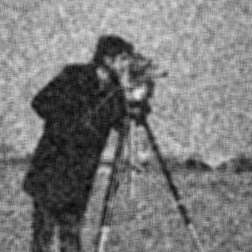
\includegraphics[width=0.9\textwidth]{../code/2_out/2-1_gaus_5x5.png}
        \caption{5x5}
        \label{fig:2-1-2:3}
    \end{subfigure}
    \begin{subfigure}[b]{0.3\textwidth}
        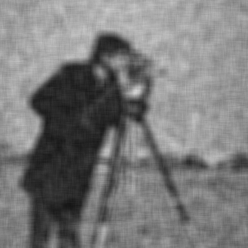
\includegraphics[width=0.9\textwidth]{../code/2_out/2-1_gaus_9x9.png}
        \caption{9x9}
        \label{fig:2-1-2:4}
    \end{subfigure}

    \caption{Averaging filter of varying sizes applied to image with gaussian noise.}
    \label{fig:2-1-2}
\end{figure}

\subsection{Code}
Code used to generate the images:
\inputminted[linenos=true]{octave}{../code/2.1.m}

\texttt{average.m}, the averaging filter function:
\inputminted[linenos=true]{octave}{../code/avgfilter.m}

\texttt{avg.m}, a function that computes the average (mean) value of a matrix:
\inputminted[linenos=true]{octave}{../code/avg.m}

\texttt{neighborhood.m}, a function that returns the \texttt{n x m} neighbourhood of a pixel at coordinates $(x,y)$ in a given image.
\inputminted[linenos=true]{octave}{../code/neighborhood.m}
